\section{Implementation}
For implementing the model, there were at least two major decisions to be made.
\begin{itemize}
    \item Which optimization software to use?
    \item What programming language to use for generating the model?
\end{itemize}
The author had previous experience with a commercial grade optimization solver
called Gurobi~\cite{gurobi}. It is advertised as a state-of-the-art
mathematical programming solver and it has a free, full-featured academic
license.

Other capable solvers for integer programming models according
to~\cite{meindl2012analysis,mittleman} are CPLEX~\cite{cplex} and XPRESS~\cite{xpress}.
However, they are also both commercial like Gurobi and Gurobi was to easiest to
get an academic licence for.

Gurobi has bindings for several languages. The ones considered were C++ and
Python. It is well known that Python as an interpreted language has a constant
runtime overhead. However, C++ has lots of unwanted complexity. The author
chose to use Python, because generating the integer programming model would
only take a fraction of the time to actually solve it. And the model solving
is not hindered by the runtime system of Python. Because there exist lots of
code that still uses version 2.X of Python, it should be explicitly
mentioned that Python 3.X was used in thesis. To be precise, the exact version
was Python 3.5.1.
\subsection{PANDA}
Programmers are used to thinking in terms of if-clauses. However, in an integer
programming model there are no ifs. At first it was hard to come up with
constraints. We knew which variables were involved and what values were legal,
but writing them as a constraint was still unintuitive. Finding the right
constraint when there were five or more variables proved hard to do by
hand. Fortunately there is a tool called PANDA~\cite{panda} to help with
finding constraints.

PANDA is short for Parallel AdjaceNcy Decomposition Algorithm and its internal
algorithm is more or less the same as Fourier-Motzkin elimination algorithm,
which is taught at the University of Tartu in the course MTAT.05.120
``Combinatorial Optimization''.

PANDA takes an input file, which list the variables and feasible values of the
variables. Then it processes this list of feasible values and outputs a
complete system of equalities and inequalities that hold between the variables.
As an example here is the contents of an valid input file.
\begin{verbatim}
Names:
occu incoming

Vertices:
0 0
1 1
1 2
\end{verbatim}
And the corresponding output by PANDA is:
\begin{verbatim}
PANDA -- facet enumeration with double description
Inequalities:
-2occu +incoming <= 0
occu -incoming <= 0
occu <= 1
\end{verbatim}

Writing input files for PANDA is a little tedious, because you have to list all
the feasible assignments of values to variables. We wrote little programs with
regular if-clauses to generate input files for PANDA. PANDA outputs lots of
inequalities, but some of them are trivial and already covered by other
constraints in the model. Therefore, human judgement was still needed to see
which inequalities and equalities added something valuable to the integer
programming model.
\subsection{Graphical visualization}
For testing the model and seeing the solutions found, we needed some kind of
feedback. At first we had a textual output of the node status and decision
variables for each timestep, it is depicted on~\autoref{fig:nogui}.

\begin{figure}[h]
    \begin{center}
	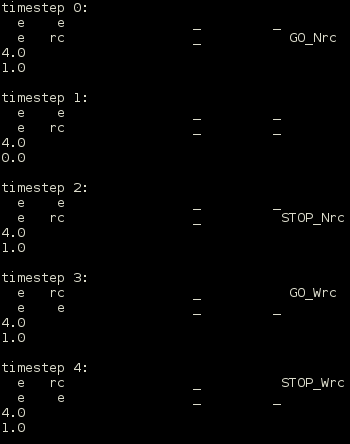
\includegraphics[scale=0.7]{fig/nogui.png}
        \caption{Early textual output of variables. On the left are the node
            statuses for a 2x2 grid and on the right are the decision variables.
        Note that the variables were different then.}
        \label{fig:nogui}
    \end{center}
\end{figure}

However, when the time came to find out, if edge occupied variables had
reasonable values in the solution, the textual output was not good enough to
display the directed edges well. Instead of improving the textual output, we
chose to implement the visualization of solutions graphically.

Because the visualization was used mostly for debugging purposes, there was not
a lot of effort and time put into writing it. To minimize the effort we wrote
the graphical visualization using the de-facto standard Python graphical user
interface package TkInter~\cite{tkinter}. The graphical visualization shows the
underlying graph of the problem one timestep at a time. There are keybindings
to increase and decrease the visible timestep. For a given timestep, the
occupied edges are highlighted. At each vertex, the node status is displayed
and if one of the decision variables was set to 1, the decision is also displayed
inside the vertex. A screenshot of the visualization graphical interface is
on~\autoref{fig:gui}.

\begin{figure}[h]
    \begin{center}
	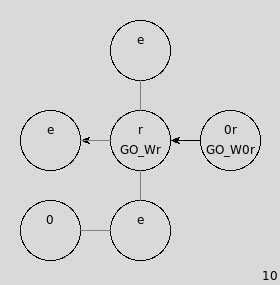
\includegraphics[scale=0.6]{fig/app/ex10.png}
        \caption{Screenshot of the graphical visualization. Circles are the
            nodes, gray lines between them show edges. Black arrows show
            occupied edges. Inside the nodes, the upper text displays the node
            status and the lower text the current decision. In the lower right
        corner is a number, which show the current timestep. }
        \label{fig:gui}
    \end{center}
\end{figure}

\subsection{Irreducible inconsistent subsystem}
In the development phase errors were made. Sometimes a feasible movement were
not feasible in the integer programming model. This would mean that all the
constraints would need to be carefully verified again. Luckily, Gurobi can
calculate an irreducible inconsistent subsystem of an infeasible model.
Inconsistent subsystem of an integer program is a subset of constraints, that
are inconsistent. Irreducible inconsistent subsystem is a minimal
inconsistent subsystem. Basically we can ask Gurobi to find out which set of
constraints make the model infeasible. After we get such a set, we only have to
recheck the constraints that are in the irreducible inconsistent subsystem.

As an example here is the irreducible inconsistent subsystem given by Gurobi
for the orthogonal collision illustration in~\autoref{sec:orthcoltest}.
\begin{verbatim}
Minimize
 
Subject To
 R432: occu(((1,0),(0,0)),0) + occu(((1,0),(2,0)),0)
   + occu(((1,1),(1,0)),0) <= 1
 R5655: - occu(((1,0),(0,0)),0) + go((1,0),'r','W',0)
   + cont((2,0),'r','W',0) <= 0
 R5792: - occu(((1,1),(1,0)),0) + go((1,1),'r','N',0) <= 0
 R6328: cont((2,0),'r','W',0) = 0
 R8494: go((1,0),'r','W',0) = 1
 R8495: go((1,1),'r','N',0) = 1
Bounds
 occu(((1,0),(0,0)),0) free
 occu(((1,1),(1,0)),0) free
 go((1,0),'r','W',0) free
 go((1,1),'r','N',0) free
 cont((2,0),'r','W',0) free
Generals
 occu(((1,0),(0,0)),0) occu(((1,0),(2,0)),0) occu(((1,1),(1,0)),0)
 go((1,0),'r','W',0) go((1,1),'r','N',0) cont((2,0),'r','W',0)
End
\end{verbatim}
\subsection{Tuning Gurobi parameters}
Gurobi might be the best mixed integer program solver around, but as the
problems are NP-complete, it still takes a long time to find the optimal
solution. Gurobi has a lot of parameters~\cite{gurobiparams} that can be
altered, which affect the total runtime. Finding a good set of parameters to
tune is a tedious task, therefore Gurobi comes with an automatic tuning tool.
The tuning tool has an API, but the easiest way is to run it from command line
as a separate tool called \textit{grbtune}.

The tuning tool will take as input integer programming models and then optimize
them many times in a row to establish a baseline performance. After the
baseline is established it will try different set of parameters and it then
outputs those sets that improved on the baseline performance.

Different objective functions leaded to different parameters. When we used
objective function~\eqref{eq:timeobj} with the terminal configuration fixed
with constraints~\eqref{eq:termcont}, \textit{grbtune} reported the following
set of parameters.
\begin{itemize}
    \item MIPFocus = 2
    \item Presolve = 2
    \item PrePasses = 3
    \item Cuts = 0
\end{itemize}

However, when I switched to objective function~\eqref{eq:objective} and
without the terminal configuration constraints, the only parameter that Gurobi
tuning tool found was:
\begin{itemize}
    \item AggFill = 5
\end{itemize}

Now we briefly explain the settings. In the first case MIPFocus is used to
controls the focus of MIP solver. Focus 2 means to work on the best bound.
Presolve controls the aggressiveness of pre-solving the model. Value of 2 means
that pre-solving is aggressive. PrePasses is used to limit the number of
pre-solving passes. Cuts = 0 turns off all cut generations. AggFill controls
the fill level in pre-solve aggregations, with larger values generally lead to
more presolved rows and columns, but at the same time leave more non-zeros in
the constraint matrix~\cite{gurobiparams}.
